\documentclass[12pt]{article}

\usepackage{sbc-template}
\usepackage{graphicx,url}
\usepackage[utf8]{inputenc}
\usepackage[brazil]{babel}
\usepackage{amsmath}
\usepackage{placeins}
\setlength{\emergencystretch}{2em}

\title{Eficiência, Justiça e Exclusão em Escalonadores 5G sob Cargas Variáveis}

\author{Alex Reis, David Hudson, Luana Teles,\\ Thiago Nerton, Victor Cleyton, Vitória Pontes}

\address{Universidade Federal do Cariri (UFCA), Juazeiro do Norte, CE, Brasil}

\begin{document}

\maketitle

\begin{resumo}
Este trabalho compara Round Robin (RR), MaxCI, operacionalizado como uma política de melhor taxa instantânea, e Proportional Fair (PF) em uma célula SISO de enlace descendente inspirada em 5G. O experimento usa 50 sementes pareadas, cinco cargas e dois regimes: UEs homogêneos e heterogeneidade espacial controlada por um modelo log-distance de perda de percurso. No cenário homogêneo, MaxCI mantém os índices de justiça de slots e de vazão próximos de 1, mas apresenta intervalos sem atendimento mais longos. Com heterogeneidade, MaxCI preserva a maior vazão agregada, porém concentra o serviço e pode excluir UEs, degradando a cauda inferior de vazão. Entre as políticas avaliadas, PF combina justiça de vazão superior à de RR no cenário heterogêneo com maior percentil inferior de vazão. Os resultados são apresentados com métricas de vazão, Jain, Gini, exclusão e robustez à definição de justiça.
\end{resumo}

\begin{abstract}
This work compares Round Robin (RR), MaxCI, operationalized as a best-instantaneous-rate policy, and Proportional Fair (PF) in a SISO downlink cell inspired by 5G. The experiment uses 50 paired seeds, five loads, and two regimes: homogeneous users and controlled spatial heterogeneity through a log-distance path-loss model. Under homogeneous channels, MaxCI retains slot and throughput fairness close to one but exhibits longer intervals without service. Under heterogeneity, MaxCI preserves the highest aggregate throughput while concentrating service. PF provides higher throughput fairness and lower-tail throughput than RR in the heterogeneous regime. Results are reported using throughput, Jain, Gini, exclusion, and robustness-to-metric measures.
\end{abstract}

\section{Introdução}

Os escalonadores de rádio (schedulers) definem qual UE recebe o recurso disponível em cada intervalo de transmissão. RR distribui os intervalos em ordem cíclica. MaxCI prioriza a melhor condição instantânea; neste trabalho, essa decisão é implementada pela maior taxa instantânea realizável. PF compara a taxa instantânea com o histórico do próprio UE. Essas escolhas colocam eficiência e justiça em tensão, mas a forma dessa tensão depende do canal e da métrica adotada \cite{jain1984quantitativemeasurefairnessdiscrimination,tse2005fundamentals}.

A literatura de escalonamento em 5G descreve RR, Max Rate/Max C/I e PF como baselines de políticas que priorizam, respectivamente, rodízio, oportunidade instantânea e compromisso com o histórico de serviço \cite{9773317}. O estudo usa Sionna para o canal de pequena escala, mas não implementa os cenários completos do TR 38.901; o ganho log-distance é uma premissa de contraste controlado, não uma simulação padronizada de propagação \cite{3gpp38901}.

A pergunta do estudo é: como carga, heterogeneidade espacial e definição de justiça alteram a comparação entre RR, MaxCI e PF? O estudo não pretende representar todos os componentes de um sistema 5G comercial; busca isolar o efeito do scheduler em um cenário controlado e identificar onde a conclusão muda quando se introduz vantagem média persistente de canal.

\section{Fundamentação teórica}

\subsection{Políticas de escalonamento}

Seja $r_{u,t}$ a taxa instantânea realizável pelo UE $u$ no TTI $t$, e seja $u_t$ o UE escolhido. As três políticas seguem regras distintas \cite{9773317}. O Round Robin (RR) ignora o estado instantâneo do canal e percorre ciclicamente os $N$ UEs; para TTIs numerados a partir de zero,
\begin{equation}
u_t=t\bmod N.
\end{equation}

O MaxCI é operacionalizado no simulador como uma política Max Rate, selecionando o UE de maior taxa instantânea realizável,
\begin{equation}
u_t=\arg\max_u r_{u,t}.
\end{equation}
Como não há interferência intercelular explícita no cenário, o nome MaxCI é mantido como rótulo da política oportunista, enquanto a decisão efetivamente implementada é feita sobre a taxa instantânea.

No Proportional Fair (PF), a taxa instantânea é normalizada pelo histórico de vazão do UE,
\begin{equation}
u_t=\arg\max_u\frac{r_{u,t}}{T_u(t)}.
\end{equation}
Após a seleção, o histórico é atualizado por média móvel exponencial,
\begin{equation}
T_u(t+1)=\beta T_u(t)+(1-\beta)\,\mathbf{1}\{u_t=u\}\,r_{u,t},
\qquad \beta=0{,}98.
\end{equation}
Na implementação, todos os históricos partem do mesmo valor positivo, evitando divisão por zero e preservando condições iniciais simétricas.

\subsection{Justiça de slots e de vazão}

O Jain's Fairness Index (JFI) para um vetor não negativo $\mathbf{x}$ é \cite{jain1984quantitativemeasurefairnessdiscrimination}
\begin{equation}
J(\mathbf{x})=\frac{(\sum_u x_u)^2}{N\sum_u x_u^2},
\end{equation}
com $J=1$ para distribuição uniforme. Neste estudo, ele é aplicado tanto aos slots quanto à vazão. Se
\begin{equation}
s_u=\sum_{t=0}^{T-1}\mathbf{1}\{u_t=u\}
\end{equation}
é o número de TTIs atribuídos ao UE $u$, então $J_{\mathrm{slots}}=J(\mathbf{s})$. Como todos os TTIs têm a mesma duração, a vazão média do UE pode ser escrita como
\begin{equation}
q_u=\frac{1}{T}\sum_{t=0}^{T-1}\mathbf{1}\{u_t=u\}\,r_{u,t},
\end{equation}
e $J_{\mathrm{vaz}}=J(\mathbf{q})$. Portanto, igualdade de oportunidades de transmissão não implica igualdade de vazão quando os UEs possuem condições médias de canal diferentes.

No cenário homogêneo, os UEs têm a mesma distribuição de canal por construção. Assim, embora MaxCI escolha a maior taxa em cada TTI, nenhum UE possui vantagem média persistente; por simetria, as oportunidades de seleção tendem a se equilibrar em horizontes longos. A introdução de ganho médio dependente da distância quebra essa simetria e permite que alguns UEs sejam favorecidos sistematicamente \cite{tse2005fundamentals}.

\section{Metodologia}

\subsection{Cenário e geração pareada}

O experimento usa uma célula SISO de enlace descendente com tráfego de buffer sempre cheio (full-buffer), cinco cargas ($N\in\{2,4,8,16,32\}$), 10.000 intervalos de transmissão (TTIs) por semente aleatória e 50 sementes por condição. O canal de pequena escala segue desvanecimento Rayleigh em blocos (block-fading) produzido por Sionna \cite{nvidiasionna2022}. A taxa instantânea realizável é
\begin{equation}
r_{u,t}=B_{\mathrm{occ}}\min\left\{\log_2(1+\gamma|h_{u,t}|^2),\eta_{\max}\right\},
\end{equation}
onde $B_{\mathrm{occ}}$ é a banda ocupada, $\gamma$ é a SNR de referência e $\eta_{\max}$ é o limite de eficiência espectral.

Cada condição usa os mesmos índices de sementes para RR, PF e MaxCI. Isso permite comparar os escalonadores sem trocar a realização de canal entre políticas. O braço homogêneo não aplica perda de percurso. Os seis cenários heterogêneos aplicam o ganho relativo
\begin{equation}
\tilde d_u=\max(d_u,d_0),\qquad
g_u=\frac{(d_0/\tilde d_u)^\alpha}{\frac{1}{N}\sum_v(d_0/\tilde d_v)^\alpha},
\qquad \alpha\in\{1.5,2.0,2.5,3.0,3.5,4.0\}.
\end{equation}
O coeficiente de canal é escalado por $\sqrt{g_u}$ porque $g_u$ representa ganho de potência, enquanto $h_{u,t}$ é um coeficiente complexo de amplitude. A normalização impõe ganho médio unitário entre os UEs, preservando a escala média de SNR do cenário ao introduzir heterogeneidade relativa. Os parâmetros executados são TTI de 1 ms, banda ocupada de 18,72 MHz, SNR de referência de 10 dB, teto de 6 bit/s/Hz, $d_0=10$ m e raio de 500 m. O modelo é uma premissa didático-experimental para introduzir contraste entre UEs próximos e distantes; não é um orçamento de enlace absoluto nem uma implementação completa do TR 38.901.

\subsection{Métricas}

Para cada seed, são registradas vazão agregada da célula, vazão média por UE, percentil 5 da vazão por UE, número de UEs nunca atendidos, intervalos internos sem atendimento entre duas alocações ao mesmo UE, JFI de slots, JFI de vazão, Gini e a família $J_\beta$. O Gini mede concentração, com zero para igualdade \cite{SHI20051925}. A família $J_\beta$ é usada como verificação de robustez; o ponto $\beta=0$ é tratado como o limite entrópico $\beta\to0$ da construção de Lan et al. \cite{lan2009axiomatictheoryfairnessnetwork}.

O arquivo \path{estudo_per_seed.csv} é o arquivo de referência. A partir dele, \path{estudo_consolidado.csv} deriva média, desvio padrão e IC95 normal das métricas. Os ICs bootstrap em \path{estudo_bootstrap_ic.csv} referem-se à média do JFI de slots do MaxCI por condição, com $B=2000$ reamostragens e percentis de 2,5\% a 97,5\%.

\section{Resultados}

\subsection{Homogeneidade não produz exclusão estrutural}

No cenário homogêneo e em $N=32$, MaxCI obteve JFI de slots de 0,9972 e JFI de vazão de 0,9971. Nenhum dos 50 seeds produziu exclusão. Portanto, aumentar a carga sozinho não fez nenhum dos JFIs de MaxCI cruzar 0,5 nesse modelo. Esse resultado é coerente com a simetria do braço homogêneo: como os UEs têm a mesma distribuição de taxa, nenhum deles possui vantagem estatística persistente na seleção oportunista. O custo aparece na regularidade temporal: o maior intervalo médio sem atendimento foi 313,5 TTIs para MaxCI, contra 32,0 em RR e 63,8 em PF.

\subsection{Heterogeneidade muda o regime de MaxCI}

A Figura~\ref{fig:jfi} compara o cenário homogêneo com o braço log-distance $\alpha=3$. No homogêneo, as três políticas permanecem próximas de justiça perfeita. No braço heterogêneo, o ganho persistente $g_u$ quebra a simetria entre UEs; MaxCI passa a favorecer com maior frequência aqueles com melhores distribuições de taxa e perde justiça de slots e de vazão à medida que a carga cresce. RR mantém igualdade de slots, mas a vazão continua desigual porque UEs distantes usam seus TTIs com taxas menores. PF mantém justiça de slots próxima de 1 e, no regime heterogêneo, apresenta JFI de vazão superior ao de RR. Em $N=32$ e $\alpha=3$, a diferença pareada PF menos RR no JFI de vazão é 0,140, com IC95 normal de aproximadamente $\pm0{,}012$.

\begin{figure}[!htbp]
\centering
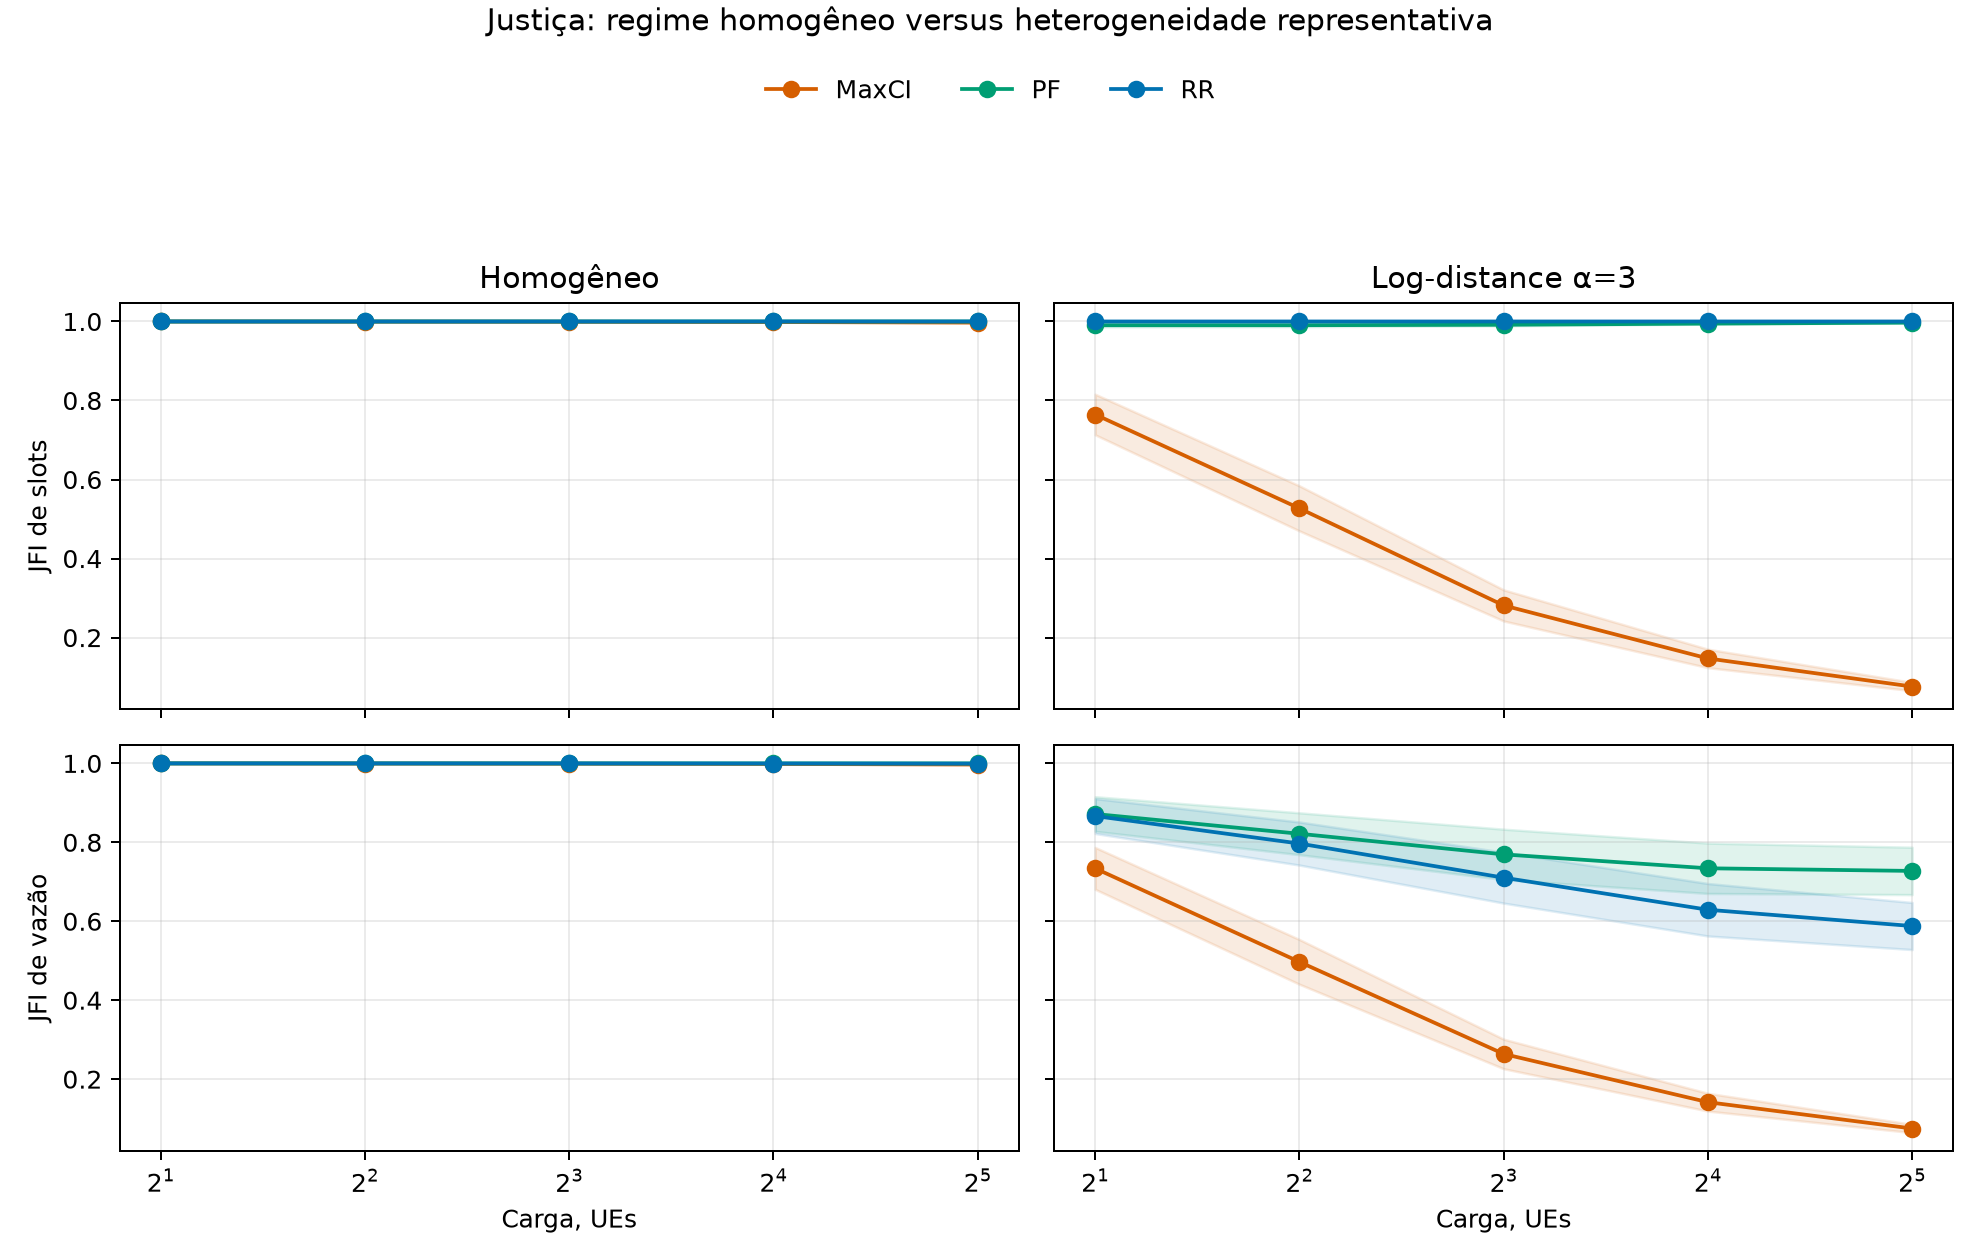
\includegraphics[width=.90\textwidth]{figuras/jfi_cenarios.png}
\caption{Justiça de slots e de vazão nos cenários homogêneo e log-distance com $\alpha=3$. As faixas representam IC95 normal entre seeds.}
\label{fig:jfi}
\end{figure}

A Tabela~\ref{tab:n32} apresenta médias de 50 seeds no maior nível de carga; os IC95 normais por métrica estão no arquivo canônico e nas figuras de carga. MaxCI mantém a maior vazão agregada, 109,41 Mbit/s no braço $\alpha=3$, mas deixa em média 19,7 dos 32 UEs sem serviço e entrega percentil 5 igual a zero. PF entrega 53,31 Mbit/s, não exclui UEs e mantém percentil 5 de 0,875 Mbit/s. RR entrega 29,26 Mbit/s e também não exclui UEs.

\begin{table}[!htbp]
\centering
\caption{Resultados em $N=32$ no cenário log-distance $\alpha=3$.}
\label{tab:n32}
\small
\begin{tabular}{lrrrrr}
\hline
Scheduler & JFI slots & JFI vazão & Vazão célula & P5 de vazão & UEs nunca atendidos \\
\hline
RR & 1,000 & 0,588 & 29,26 & 0,371 & 0,0 \\
PF & 0,997 & 0,728 & 53,31 & 0,875 & 0,0 \\
MaxCI & 0,076 & 0,075 & 109,41 & 0,000 & 19,7 \\
\hline
\end{tabular}
\end{table}

Vazão de célula e P5 estão em Mbit/s. A Figura~\ref{fig:tradeoff} mostra que, em $N=32$, a heterogeneidade reduz a justiça de vazão sobretudo para MaxCI, enquanto sua vazão agregada aumenta; a figura não identifica geograficamente quais UEs ocupam a cauda.

\begin{figure}[!htbp]
\centering
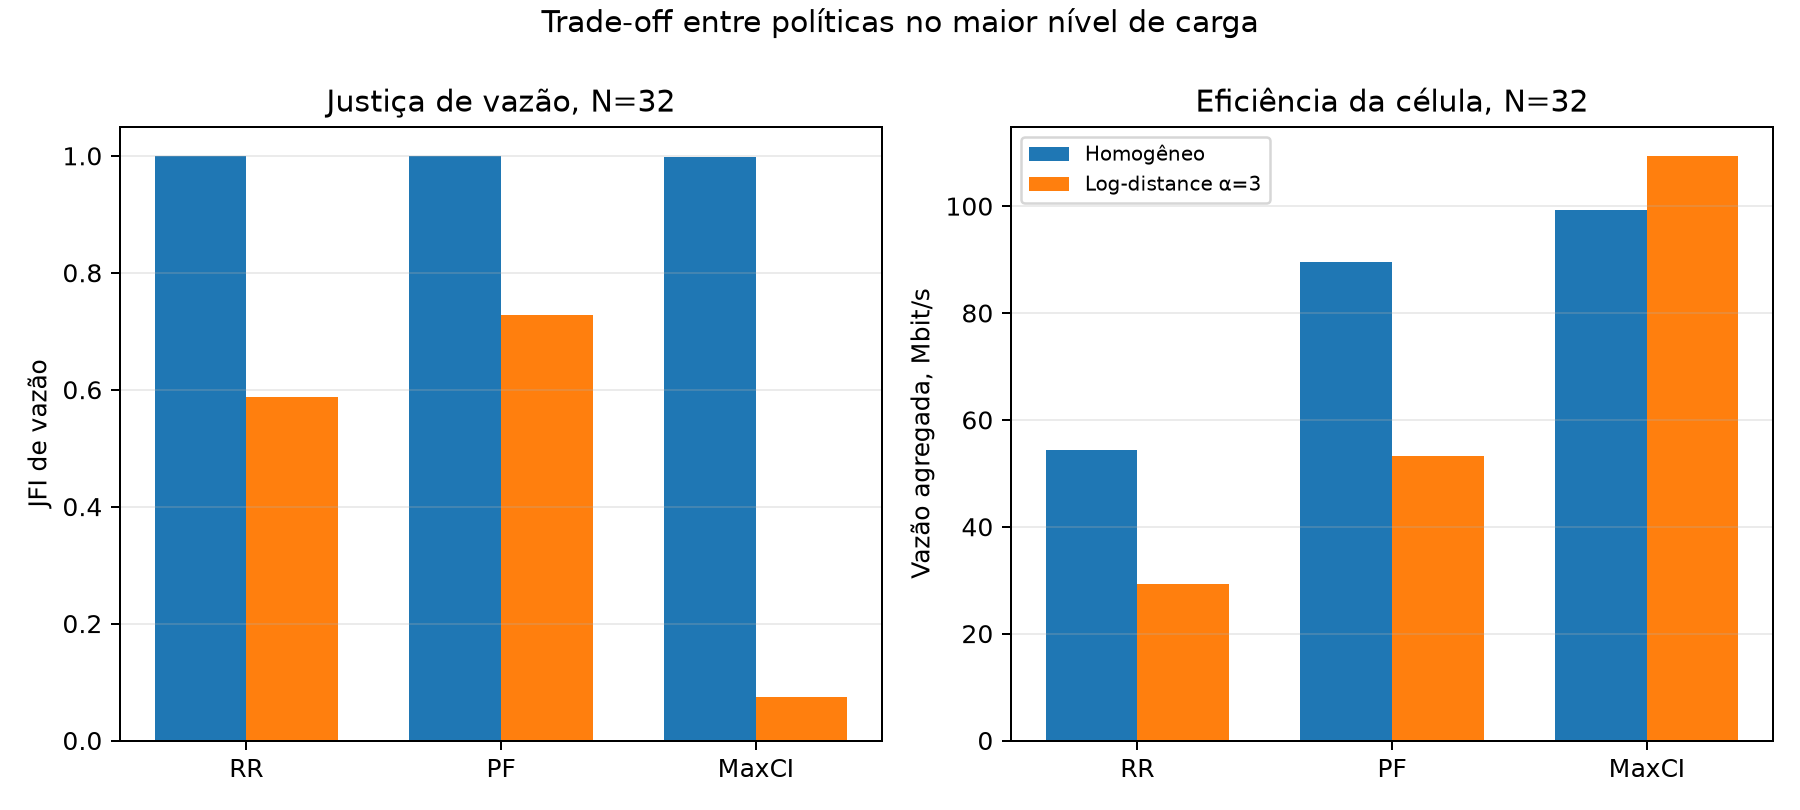
\includegraphics[width=.82\textwidth]{figuras/tradeoff_n32.png}
\caption{Compromisso entre justiça de vazão e vazão agregada em $N=32$.}
\label{fig:tradeoff}
\end{figure}

\FloatBarrier
\subsection{Severidade da heterogeneidade e robustez da conclusão}

Na Figura~\ref{fig:alpha}, para cada carga, valores maiores de $\alpha$ reduzem o JFI de slots e elevam o Gini; ambos os efeitos se acentuam com a carga. A conclusão não depende apenas do JFI: em $N=32$ e $\alpha=3$, MaxCI apresenta Gini de slots de 0,923, enquanto RR e PF apresentam 0,001 e 0,026, respectivamente. Na família $J_\beta$ aplicada aos slots, MaxCI permanece abaixo de RR e PF para todos os valores de $\beta$ avaliados; RR e PF permanecem próximos de 1.

\begin{figure}[!htbp]
\centering
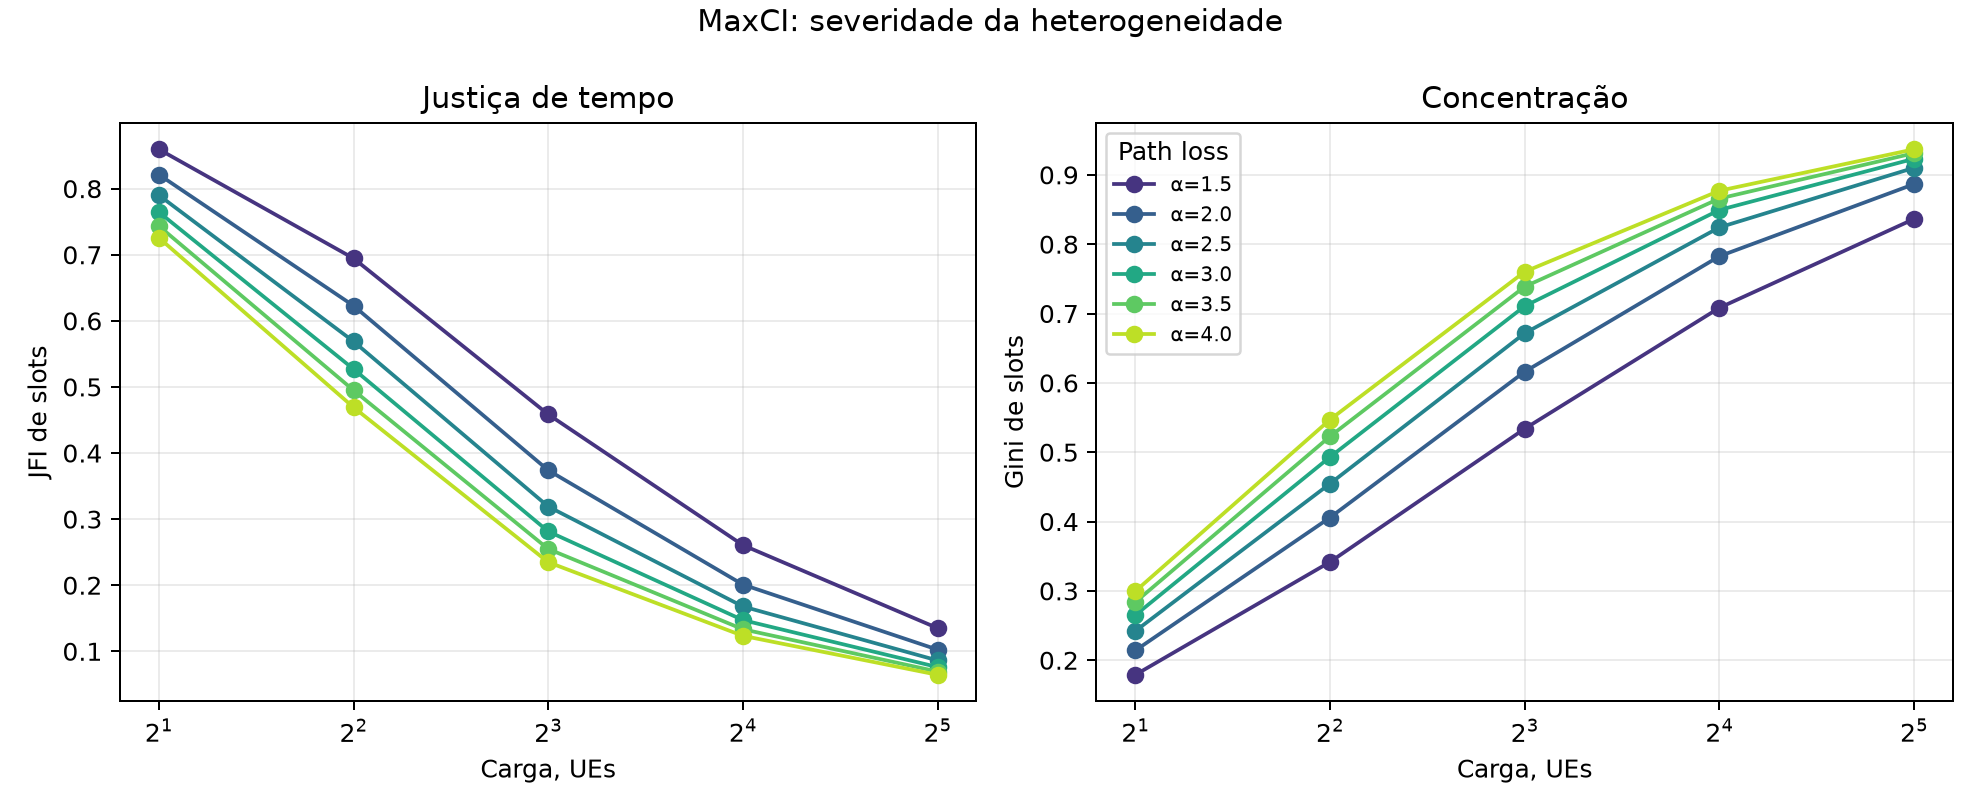
\includegraphics[width=.82\textwidth]{figuras/maxci_alpha.png}
\caption{Efeito de $\alpha$ sobre justiça e concentração do MaxCI.}
\label{fig:alpha}
\end{figure}

\begin{figure}[!htbp]
\centering
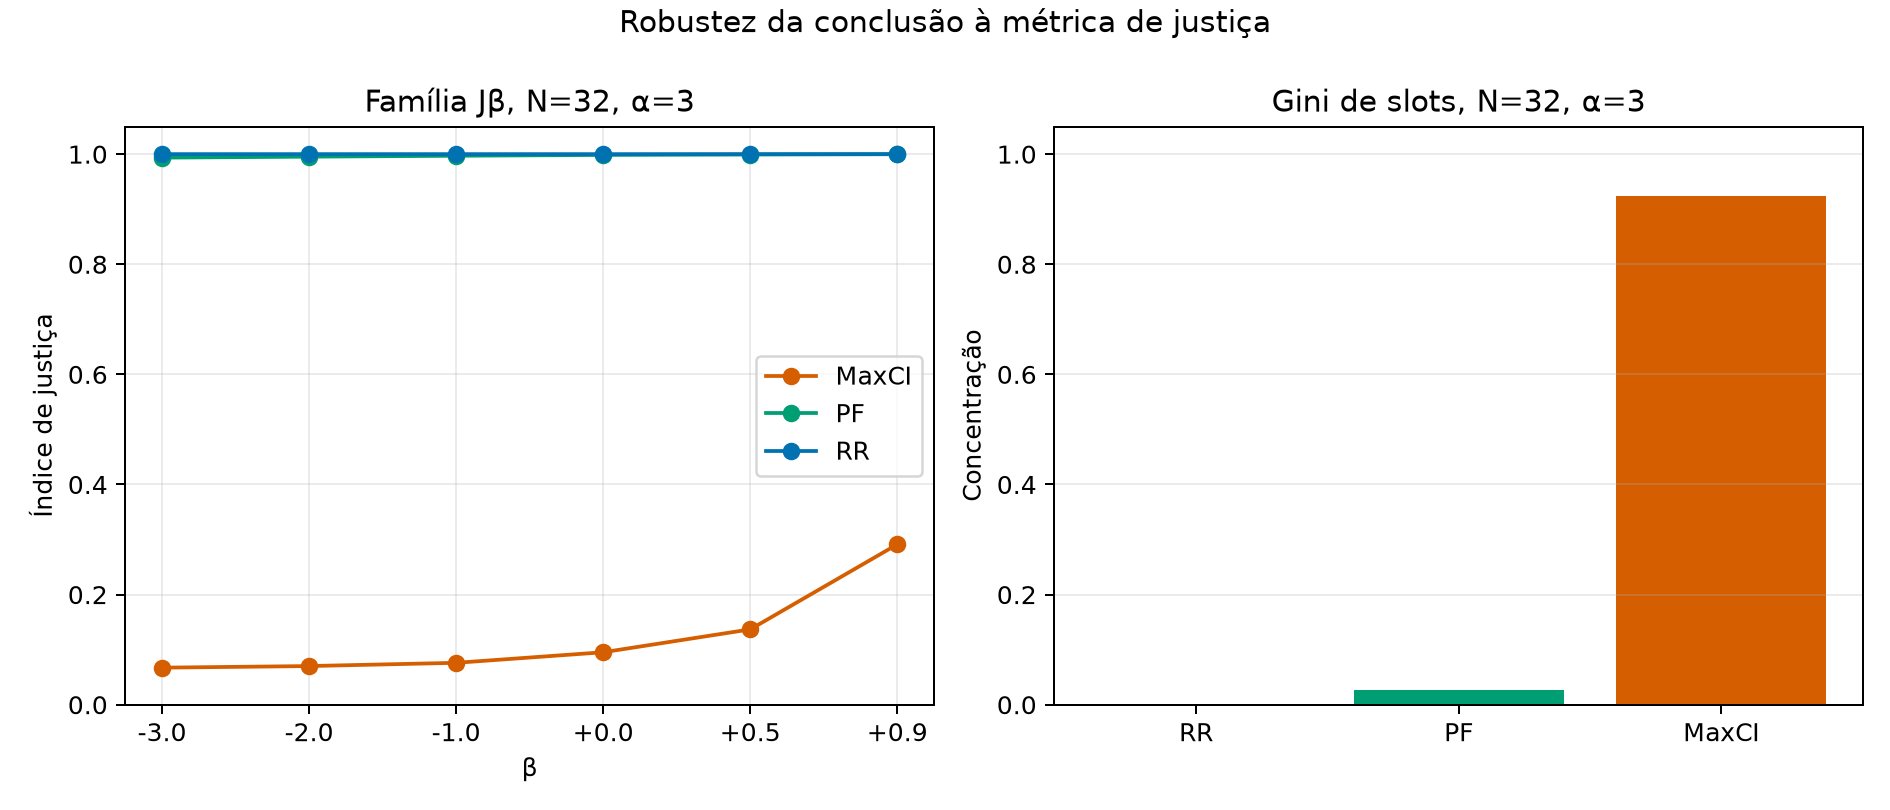
\includegraphics[width=.82\textwidth]{figuras/robustez_metricas.png}
\caption{Robustez da comparação entre políticas a diferentes métricas de justiça, em $N=32$ e $\alpha=3$.}
\label{fig:robustez}
\end{figure}

\FloatBarrier
\section{Limitações e conclusão}

Os resultados são condicionados à célula única SISO, tráfego de buffer sempre cheio (full-buffer), taxa Shannon limitada e modelo relativo de heterogeneidade. O modelo log-distance não inclui shadowing, interferência intercelular, HARQ, mobilidade ou orçamento de enlace completo. Além disso, os intervalos sem atendimento reportados são internos entre duas alocações, portanto devem ser interpretados junto com o número de UEs nunca atendidos.

Uma limitação adicional da implementação é o desempate no MaxCI. Como a taxa é limitada a 6 bit/s/Hz, podem ocorrer empates exatos no valor máximo; a operação \texttt{argmax} usada no código escolhe o primeiro índice em caso de empate. A política continua selecionando uma taxa máxima, mas essa regra pode acentuar a concentração entre UEs empatados. Assim, os valores quantitativos de exclusão devem ser interpretados como condicionados também a esse mecanismo de desempate.

Nos experimentos realizados, carga sozinha não produz colapso de justiça agregada em MaxCI quando os UEs têm a mesma distribuição de SNR. A heterogeneidade persistente altera essa conclusão: MaxCI aumenta a vazão total, mas concentra o aumento de vazão em poucos UEs. RR elimina a exclusão total medida por UEs nunca atendidos, mas mantém gaps regulares de serviço e não equaliza vazão. Entre as políticas avaliadas, PF combinou justiça de vazão superior à de RR no cenário heterogêneo com maior percentil inferior de vazão.

\bibliographystyle{sbc}
\bibliography{referencias}

\end{document}
